\section{随机事件及其概率}

\subsection{事件的运算}

\begin{theorem}[交换律]
    $\sj{A} \cup \sj{B}=\sj{B} \cup \sj{A},~\sj{A} \sj{B}=\sj{B} \sj{A} .$
\end{theorem}

\begin{theorem}[结合律]
    $\sj{A} \cup \sj{B} \cup \sj{C}=(\sj{A} \cup \sj{B}) \cup \sj{C}=\sj{A} \cup(\sj{B} \cup \sj{C}),~\sj{A} \sj{B} \sj{C}=(\sj{A} \sj{B}) \sj{C}=\sj{A}(\sj{B} \sj{C}) .$\\
    特别地 $(\sj{A} \cup \sj{B}) \cap \sj{C}=\sj{A} \cup(\sj{B} \cap \sj{C})$ 不一定成立,比如当 $ \sj{A} \neq \varnothing,~\sj{B}=\Omega,~\sj{C}=\varnothing $ 时,该式不成立.
\end{theorem}

\begin{theorem}[和与积的分配律]
    $(\sj{A} \cup \sj{B}) \cap \sj{C}=(\sj{A} \cap \sj{C}) \cup(\sj{B} \cap \sj{C}),~(\sj{A} \cap \sj{B}) \cup \sj{C}=(\sj{A} \cup \sj{C}) \cap(\sj{B} \cup \sj{C}) .$
\end{theorem}

\begin{theorem}[差与积的分配律]
    $(\sj{A}-\sj{B}) \cap \sj{C}=(\sj{A} \cap \sj{C})-(\sj{B} \cap \sj{C}),~(\sj{A} \cap \sj{B})-\sj{C}=(\sj{A}-\sj{C}) \cap(\sj{B}-\sj{C}) .$
\end{theorem}

\begin{theorem}[和与差的分配律]
    $(\sj{A} \cup \sj{B})-\sj{C}=(\sj{A}-\sj{C}) \cup(\sj{B}-\sj{C})$\\
    特别地 $(\sj{A}-\sj{B}) \cup \sj{C}=(\sj{A} \cup \sj{C})-(\sj{B} \cup \sj{C})$ 不一定成立,比如当 $ \sj{A}=\sj{B},~\sj{C} \neq \varnothing $ 时,该式不成立.
\end{theorem}

\begin{theorem}[对偶律]
    $\overline{\sj{A} \cup \sj{B}}=\bar{\sj{A}} \bar{\sj{B}},~\overline{\sj{A} \sj{B}}=\bar{\sj{A}} \cup \bar{\sj{B}},~\overline{\sj{A} \cup \sj{B} \cup \sj{C}}=\bar{\sj{A}} \bar{\sj{B}} \bar{\sj{C}},~\overline{\sj{A} \sj{B} \sj{C}}=\bar{\sj{A}} \cup \bar{\sj{B}} \cup \bar{\sj{C}} .$
\end{theorem}

\begin{theorem}[和差转换]
    \begin{enumerate}[label=(\arabic{*})]
        \item 差: $\sj{A}-\sj{B}=\begin{cases}
                      \sj{A}-\sj{A} \sj{B}=\sj{A} \bar{\sj{B}} \\ \sj{A}-\sj{B} \sj{A}=\bar{\sj{B}} \sj{A}.
                  \end{cases}$
        \item 和: $\sj{A} \cup \sj{B}=\begin{cases}
                      (\sj{A}-\sj{B}) \cup \sj{B}=\sj{A} \bar{\sj{B}} \cup \sj{B}=\bar{\sj{B}} \sj{A} \cup \sj{B} \\ \sj{A} \cup(\sj{B}-\sj{A})=\sj{A} \cup \bar{\sj{A}} \sj{B}=\sj{A} \cup \sj{B} \bar{\sj{A}}.
                  \end{cases}$
    \end{enumerate}
\end{theorem}

\subsection{概率的性质}

\begin{theorem}
    $P(\varnothing)=0,~ P(\Omega)=1 .$
\end{theorem}

\begin{theorem}[有限可加性]
    设 $ \sj{A}_{1},~\sj{A}_{2},~\cdots,~\sj{A}_{n} $ 是两两互不相容的事件,则有
    $$P\left(\sj{A}_{1} \cup \sj{A}_{2} \cup \cdots \cup \sj{A}_{n}\right)=P\left(\sj{A}_{1}\right)+P\left(\sj{A}_{2}\right)+\cdots+P\left(\sj{A}_{n}\right)$$
    \begin{enumerate}[label=(\arabic{*})]
        \item 事件 $\sj{S}$ 被分成两个不相容的事件 $\sj{S}_{1},~\sj{S}_{2}\left(\sj{S}_{1} \sj{S}_{2}=\varnothing,~\sj{S}_{1} \cup \sj{S}_{2}=\sj{S}\right)$,
        则 $ P(\sj{S})=P\left(\sj{S}_{1}\right)+P\left(\sj{S}_{2}\right)$;
        \item 若 $ \sj{S}_{1} \subset \sj{S}$,则 $ P\left(\sj{S}-\sj{S}_{1}\right)=P(\sj{S})-P\left(\sj{S}_{1}\right).$
    \end{enumerate}
\end{theorem}

\begin{theorem}[求逆公式]
    $P\qty(\bar{\sj{A}})=1-P(\sj{A}).$
\end{theorem}

\begin{example}
    设 $\sj{A},\sj{B}$ 为两个随机事件,若 $P(\sj{AB})=0.25,~P(\sj{B})=0.3,~P(\sj{A}\cup\sj{B})=0.6$,求 $P\qty(\sj{A}\mid\overline{\sj{B}})$.
\end{example}
\begin{solution}
    如图 \ref{figures/ven1.pdf} 所示,则 $P\qty(\sj{A}\mid\overline{\sj{B}})=\dfrac{P\qty(\sj{A\overline{B}})}{P\qty(\overline{\sj{B}})}=\dfrac{0.3}{1-P(\sj{B})}=\dfrac{3}{7}.$
\end{solution}

\begin{minipage}[b]{0.3\linewidth}
    \begin{figure}[H]
        \centering
        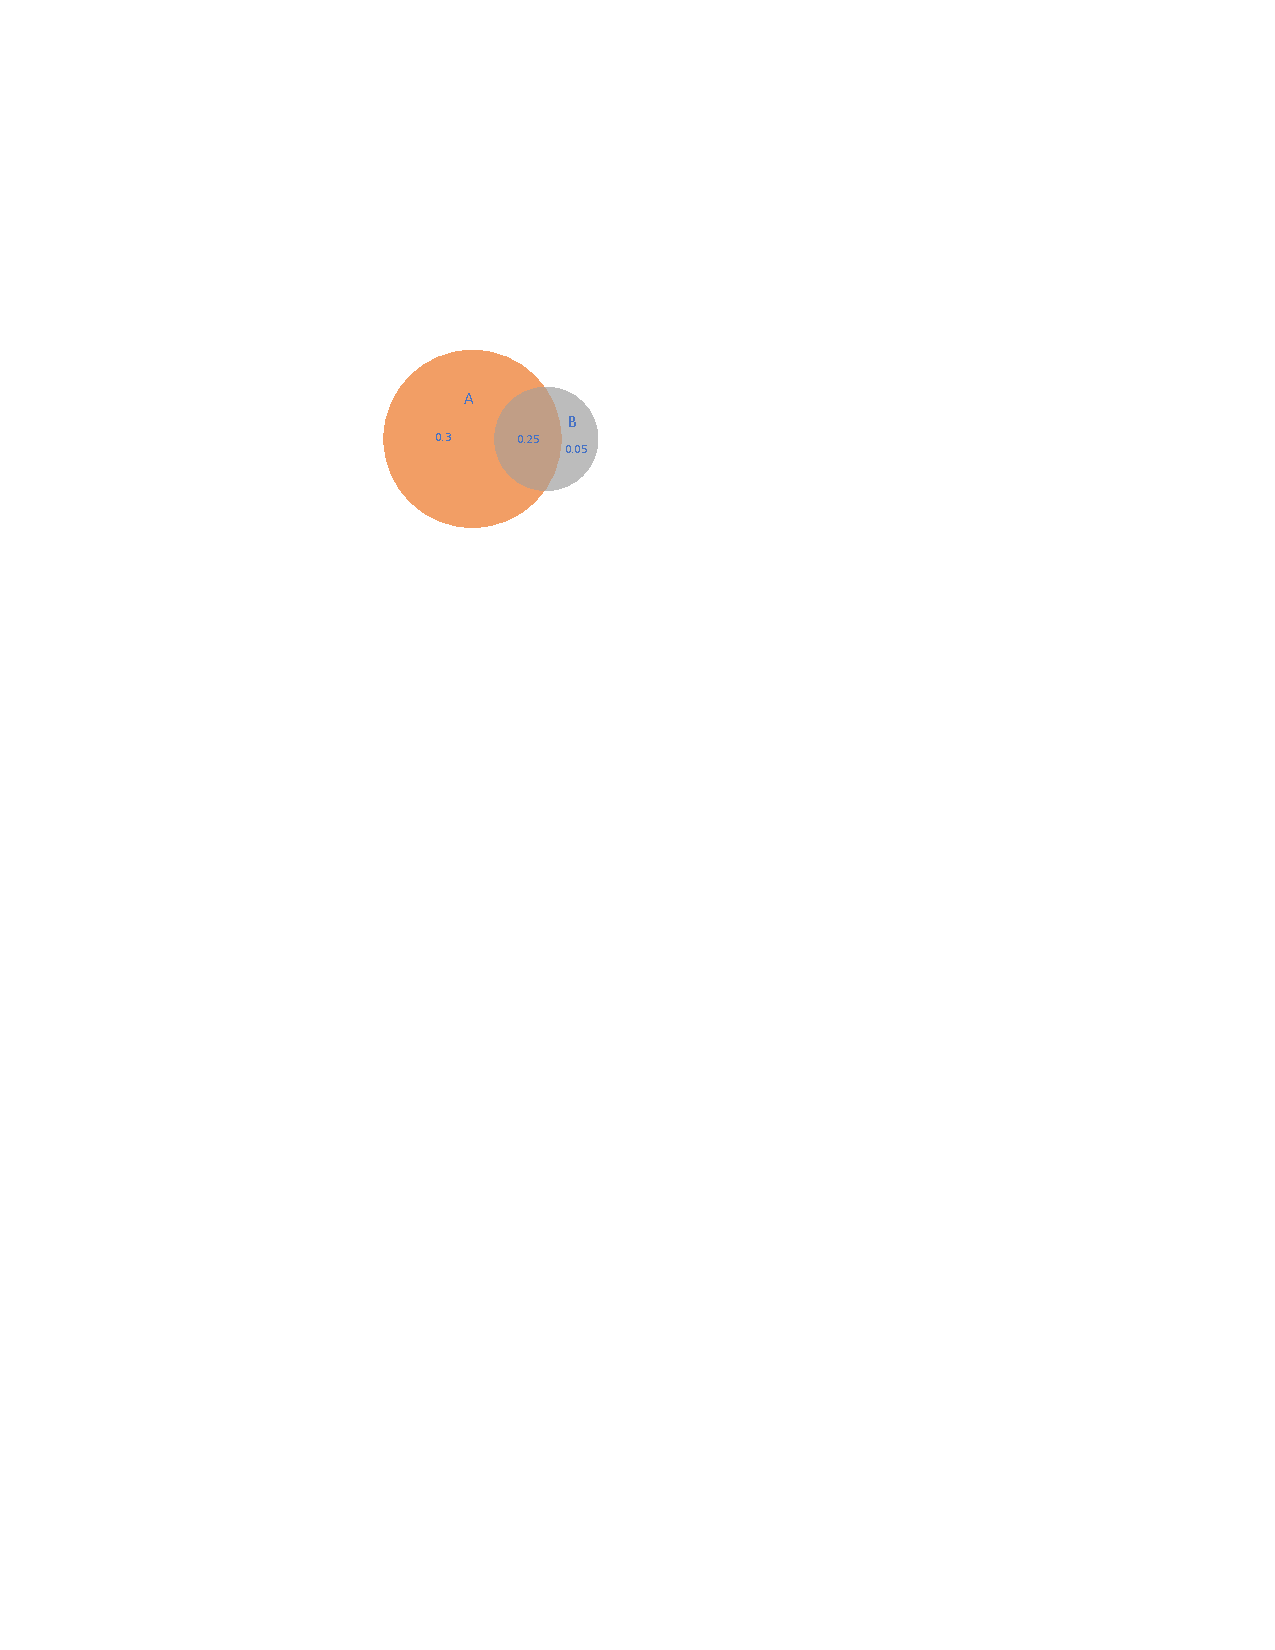
\includegraphics[scale=0.8]{figures/ven1.pdf}
        \caption{}
        \label{figures/ven1.pdf}
    \end{figure}
\end{minipage}\hfill
\begin{minipage}[b]{0.3\linewidth}
    \begin{figure}[H]
        \centering
        
\includegraphics[scale=0.8]{figures/ven2.pdf}
        \caption{}
        \label{figures/ven2.pdf}
    \end{figure}
\end{minipage}\hfill
\begin{minipage}[b]{0.3\linewidth}
    \begin{figure}[H]
        \centering
        
\includegraphics[scale=0.8]{figures/ven3.pdf}
        \caption{}
        \label{figures/ven3.pdf}
    \end{figure}
\end{minipage}

\begin{example}
    设 $\sj{A},\sj{B}$ 为随机事件,$\sj{AB}=\overline{\sj{A}}~\overline{\sj{B}},~0<P(\sj{B})<1$,求 $P\qty(\sj{A}\mid\overline{\sj{B}})+P\qty(\overline{\sj{A}}\mid\sj{B}).$
\end{example}
\begin{solution}
    因为 $\sj{AB}=\overline{\sj{A}}~\overline{\sj{B}}$,所以事件 $\sj{A}+\sj{B}=\Omega$,如图 \ref{figures/ven2.pdf} 所示,
    则 $P\qty(\sj{A}\mid\overline{\sj{B}})+P\qty(\overline{\sj{A}}\mid\sj{B})=P(\sj{A}\mid\sj{A})+P(\sj{B}\mid\sj{B})=1+1=2.$
\end{solution}

\begin{example}
    已知 $P\qty(\overline{\sj{A}})=0.3,~P(\sj{B})=0.4,~P(\sj{A}-\sj{B})=0.5$,求 $P\qty{\sj{B}\mid \qty(\sj{A}\cup\overline{\sj{B}})}.$
\end{example}
\begin{solution}
    由题意可作出如图 \ref{figures/ven3.pdf} 所示的 ven 图,则 $P\qty{\sj{B}\mid \qty(\sj{A}\cup\overline{\sj{B}})}=\dfrac{P\qty(\sj{B}\cap\qty(\sj{A}\cup\overline{\sj{B}}))}{P\qty(\sj{A}\cup\overline{\sj{B}})}=\dfrac{P(\sj{AB})}{1-P(\sj{AB})}=0.25.$
\end{solution}

% 子性质三:  
% 子性质四:  P(\sj{A} \bar{\sj{B}})=P(\sj{A})-P(\sj{A} \sj{B})  (减法公式)
% 性质三 (减法公式):  P(\sj{A}-\sj{B})=P(\sj{A} \bar{\sj{B}})=P(\sj{A})-P(\sj{A} \sj{B}) 
% 若  \sj{B} \subset \sj{A},~P(\sj{A}-\sj{B})=P(\sj{A})-P(\sj{B}) 
% 若  \sj{A} \sj{B}=\varnothing,~P(\sj{A}-\sj{B})=P(\sj{A}) 
% 性质四 (加法公式):  P(\sj{A} \cup \sj{B})=P(\sj{A})+P(\sj{B})-P(\sj{A} \sj{B}) 
%  P(\sj{A} \cup \sj{B} \cup C)=P(\sj{A})+P(\sj{B})+P(C)-P(\sj{A} \sj{B})-P(\sj{A} C)-P(\sj{B} C)+P(\sj{A} \sj{B} C) 
% 证明:  P(\sj{A} \sj{B})+P(\sj{A} C)+P(\sj{B} C)+1 \geqslant P(\sj{A})+P(\sj{B})+P(C) 
% 性质五:  P(\sj{A} \sj{B})=P(\sj{A}) \Leftrightarrow P(\sj{A} \cup \sj{B})=P(\sj{B}) \Leftrightarrow P(\sj{A}-\sj{B})=0 
% 性质六:  P(\sj{A} \sj{B})=0 \Leftrightarrow P(\sj{A} \bar{\sj{B}})=P(\sj{A}) \Leftrightarrow P(\sj{B} \bar{\sj{A}})=P(\sj{B}) 
% 有关不等式的性质
% 性质七:  0 \leqslant P(\sj{A}) \leqslant 1 
% 性质入: 若  \sj{S} \subset T ,~则  P(\sj{S}) \leqslant P(T) 
% 子性质一:  P(\sj{A} \sj{B}) \leqslant P(\sj{A}),~P(\sj{B}) \leqslant P(\sj{A} \cup \sj{B}),~P(\sj{A} \sj{B}) \leqslant \frac{P(\sj{A})+P(\sj{B})}{2} \leqslant P(\sj{A} \cup \sj{B}) 
% 子性质二:
% 
% \begin{array}{l}
% P(\sj{A})=0 \Rightarrow\left\{\begin{array}{l}
% P(\sj{A} \sj{B})=0 \\
% P(\sj{A} \cup \sj{B})=P(\sj{B})
% \end{array}\right. \\
% P(\sj{A})=1 \Rightarrow\left\{\begin{array}{l}
% P(\sj{A} \cup \sj{B})=1 \\
% P(\sj{A} \sj{B})=P(\sj{B})
% \end{array}\right. \\
% P(\sj{A} \sj{B})=1 \Rightarrow P(\sj{A})=P(\sj{B})=1
% \end{array}


\subsection{古典概率与几何概率}

\subsubsection{古典概率}

\begin{example}
    求 10 个不同规格的零件中混入 3 个次品,现进行逐个检查,则查完 5 个零件时正好查出 3 个次品的概率.
\end{example}
\begin{solution}
    \textbf{法一: }记 $\mathsf{A}=\text{查完 5 个零件正好查出 3 个次品}$,那么事件 $\mathsf{A}$ 由两个事件构造: $$\mathsf{B}=\text{前 4 次检查,查出 2 个次品},\mathsf{C}=\text{第 5 次检查,查出的是次品}$$
    即 $\mathsf{A}=\mathsf{BC}$,由乘法公式 $P(\mathsf{A})=P(\mathsf{BC})=P(\mathsf{B})P(\mathsf{C}|\mathsf{B})$,前 4 次检查中有 2 个正品和 2 个次品的组合为
    $$P(\mathsf{B})=\dfrac{\C_3^2\cdot\C_7^2}{\C_{10}^4}=\dfrac{3}{10}$$
    已知 $\mathsf{B}$ 发生的条件下,剩下 6 个零件中查出 1 个次品的概率为 $\dfrac{1}{6}$,即 $P(\mathsf{C}|\mathsf{B})=\dfrac{1}{6}$,于是 $P(\mathsf{A})=\dfrac{3}{10}\times\dfrac{1}{6}=\dfrac{1}{20}.$\\
    \textbf{法二: }事件 $\sj{A}$ 等价于在 3 个次品中选一个放在第 5 个位置上,然后在 7 个正品中选 2 个与余下的 2 个次品排在前 4 个位置上,最后将其余 5 个正品随意排在后面 5 个位置上,所以
    $$P(\sj{A})=\dfrac{\C_3^1\C_7^2\C_2^2\cdot 4!\cdot5!}{10!}=\dfrac{1}{20}.$$
    \textbf{法三: }考虑 3 只次品在 10 次检查中的位置,问题转化为前 4 个位置中选 2 个放次品,第 5 个位置必须放次品,于是 $$P(\sj{A})=\dfrac{\C_4^2\cdot1}{\C_{10}^3}=\dfrac{1}{20}.$$
    \textbf{法四:}只考虑放正品的位置,则前 4 个位置需要放 2 个正品,后 5 个位置全为正品,则 $P(\sj{A})=\dfrac{\C_4^2\C_5^5}{\C_{10}^3}=\dfrac{1}{20}$
\end{solution}

\subsubsection{几何概率}

\subsection{概率基本公式及条件概率}

\begin{theorem}[与独立有关的条件概率]
    设 $P(\sj{B})\in(0,1)$,则 $\sj{A} $ 与 $\sj{B}$ 相互独立的充要条件为:
    \begin{enumerate}[label=(\arabic{*})]
        \item $P(\sj{A}\mid\sj{B})=P\qty(\sj{A}\mid \bar{\sj{B}})$;
        \item $P(\sj{A}\mid\sj{B})+P\qty(\bar{\sj{A}}\mid \bar{\sj{B}})=1$;
        \item $P\qty(\bar{\sj{A}}\mid \sj{B})+P\qty(\sj{A}\mid \bar{\sj{B}})=1$.
    \end{enumerate}
\end{theorem}

\subsection{全概率公式和 Bayes 公式}

\begin{definition}[完备事件组]
    设 $ \sj{B}_{1}, \sj{B}_{2}, \cdots, \sj{B}_{n} $ 为试验 $ E $ 的一组事件,$\Omega $ 为样本空间,若满足以下两个条件:
    \begin{enumerate}[label=(\arabic{*})]
        \item $\sj{B}_{i} \sj{B}_{j}=\emptyset, i \neq j, i, j=1,2, \cdots, n $;
        \item $\sj{B}_{1} \cup \sj{B}_{2} \cup \cdots \cup \sj{B}_{n}=\Omega $.
    \end{enumerate}
    则称 $ \sj{B}_{1}, \sj{B}_{2} \cdots, \sj{B}_{n} $ 是一个完备事件组,也称 $ \sj{B}_{1}, \sj{B}_{2}, \cdots, \sj{B}_{n} $ 为样本空间 $ \Omega $ 的一个划分.
\end{definition}

\begin{theorem}[全概率公式与 Bayes 公式]
    设 $ \Omega $ 为试验 $ E $ 的样本空间,$\sj{B}_{1}, \sj{B}_{2}, \cdots, \sj{B}_{n} $ 为 $ \Omega $ 的一个划分,且 $ P\left(\sj{B}_{i}\right)>0~~(i=1,2, \cdots, n) $,则
    \begin{flalign*}
    P(\sj{A})=\sum_{i=1}^{n} P\left(\sj{B}_{i}\right) P\left(\sj{A} \mid \sj{B}_{i}\right) 
    =P\left(\sj{A} \mid \sj{B}_{1}\right) P\left(\sj{B}_{1}\right)+P\left(\sj{A} \mid \sj{B}_{2}\right) P\left(\sj{B}_{2}\right)+ 
    \cdots+P\left(\sj{A} \mid \sj{B}_{n}\right) P\left(\sj{B}_{n}\right)
    \end{flalign*}
    称为全概率公式. 而
    $$P\left(\sj{B}_{i} \mid \sj{A}\right)=\frac{P\left(\sj{B}_{i} \sj{A}\right)}{P(\sj{A})}=\frac{P\left(\sj{A} \mid \sj{B}_{i}\right) P\left(\sj{B}_{i}\right)}{\displaystyle\sum_{j=1}^{n} P\left(\sj{A} \mid \sj{B}_{j}\right) P\left(\sj{B}_{j}\right)}~~(i=1,2, \cdots, n)  $$
    称为 Bayes 公式.
\end{theorem}

\begin{example}
    一条生产线生产 $n$ 件产品不出故障的概率为 $\dfrac{\lambda^n}{n!}\e^{-\lambda}~~(n=0,1,\cdots)$ 若每件产品合格的概率为 $p~~(0<p<1)$,且各产品是否合格相互独立,
    求该生产线在两次故障之间共生产 $k~~(k=0,1,\cdots)$ 件合格品的概率.
\end{example}
\begin{solution}
    设事件 $\sj{A}_i=$“两次故障之间生产的产品总个数为 $i~~(i=0,1,\cdots)$”,事件 $\sj{B}_k=$“两次故障之间生产的合格品个数为 ”$k~~(k=0,1,\cdots,i)$,那么事件 $\sj{B}_k$ 的概率为
    \begin{flalign*}
        P\qty{\sj{B}_k} & =\sum_{i=0}^{\infty}P\qty{\sj{A}_i}\cdot P\qty{\sj{B}_k\mid \sj{A}_i}=\sum_{i=k}^{\infty}P\qty{\sj{A}_i}\cdot P\qty{\sj{B}_k\mid \sj{A}_i}=\sum_{i=k}^{\infty}\qty(\dfrac{\lambda^i}{i!}\e^{-\lambda})\cdot\qty[\C_i^kp^k(1-p)^{i-k}]                           \\
                        & =\e^{-\lambda}p^k\sum_{i=k}^{\infty}\dfrac{\lambda^i}{i!}\C_i^k(1-p)^{i-k}=\e^{-\lambda}p^k\sum_{i=0}^{\infty}\dfrac{\lambda^{i+k}}{(i+k)!}\C_{i+k}^k(1-p)^{i}=\e^{-\lambda}p^k\lambda^k\sum_{i=0}^{\infty}\dfrac{\lambda^i}{(i+k)!}\dfrac{(i+k)!}{k!i!}(1-p)^i \\
                        & =\dfrac{1}{k!}\e^{-\lambda}p^k\lambda^k\sum_{i=0}^{\infty}\dfrac{\qty[\lambda(1-p)]^i}{i!}=\dfrac{1}{k!}\e^{-\lambda}p^k\lambda^k\cdot\eval{\e^x}_{x=\lambda(1-p)}=\e^{-\lambda p}\dfrac{(p\lambda)^k}{k!}
    \end{flalign*}
\end{solution}